\subsection{Api}
	La componente \textit{Api} è il core dell'architettura; permette all'applicazione web di interfacciarsi con i due database che sono stati menzionati precedentemente, oltre che con un bot Telegram.
	La componente è stata sviluppata in Java 11 usando del framework Spring: Spring boot, Spring security, Spring kafka e Spring jpa. Per l'autenticazione web è stato usato Json Web Token.

	\subsubsection{Diagramma dei package}%%%%%%%%%%%%%%OK
		\begin{figure}[H]
			\centering
			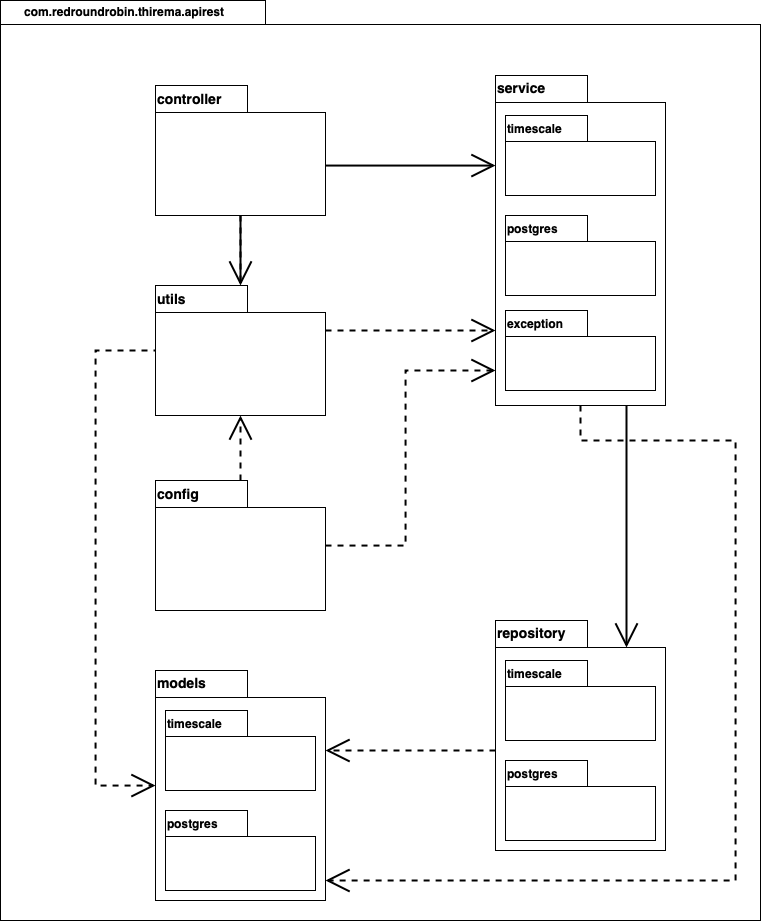
\includegraphics[scale=0.500]{res/images/API/packageAPI.png}
			\caption{Diagramma dei packages per la componente Api}
		\end{figure}

	\subsubsection{Diagrammi delle classi}%%%%%%%%%%%%%%%%%%%%%%%%%%%%%%%%%OK
		Al fine di semplificare la comprensione delle dipendenze della componente Api, si è deciso di suddividere i diagrammi per package, mostrando in dettaglio quelli più significativi.

		
		\begin{figure}[H]
			\centering
			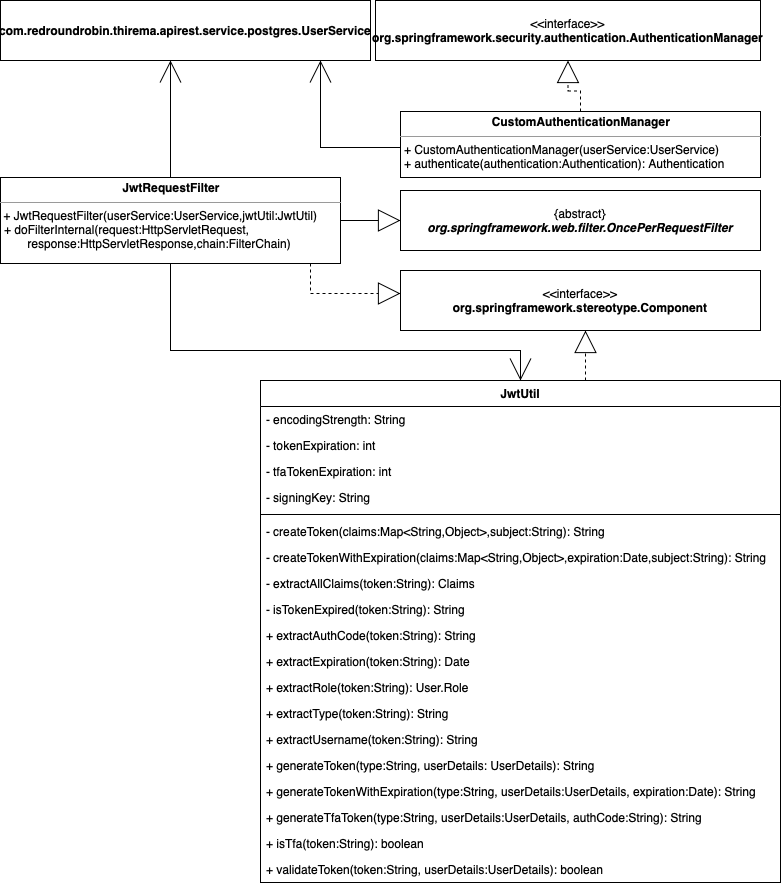
\includegraphics[scale=0.550]{res/images/API/UtilsPackage.png}
			\caption{Diagramma del package Utils della componente Api}
		\end{figure}
		\begin{figure}[H]
			\centering
			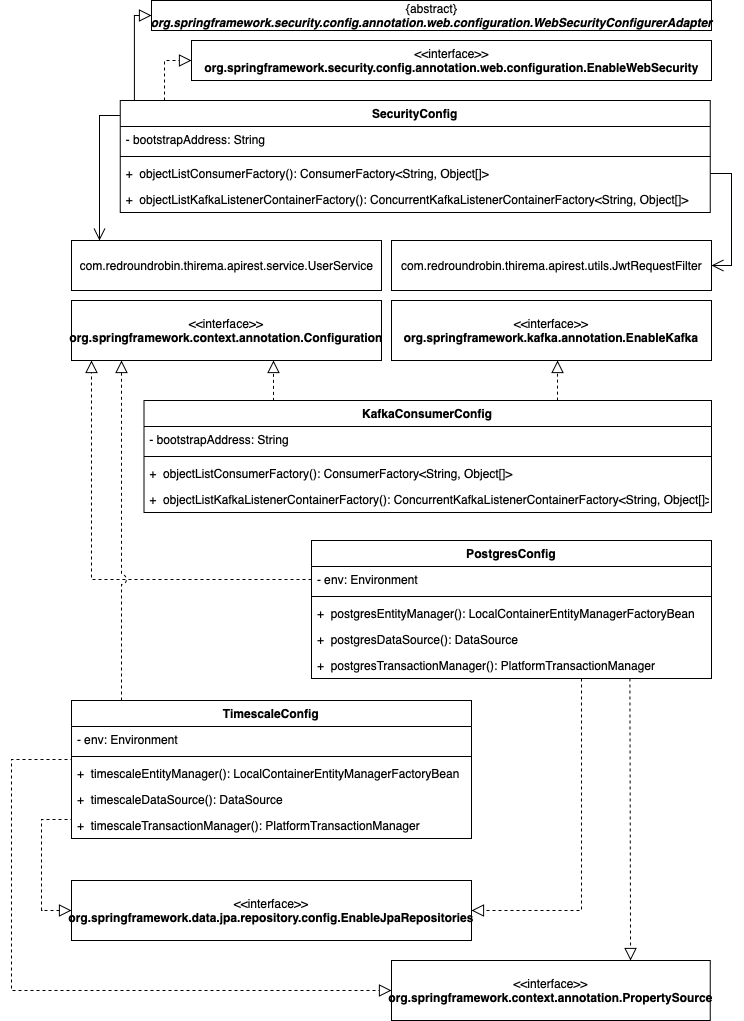
\includegraphics[scale=0.550]{res/images/API/ConfigPackage.png}
			\caption{Diagramma del package Config della componente Api}
		\end{figure}
		\begin{figure}[H]
			\centering
			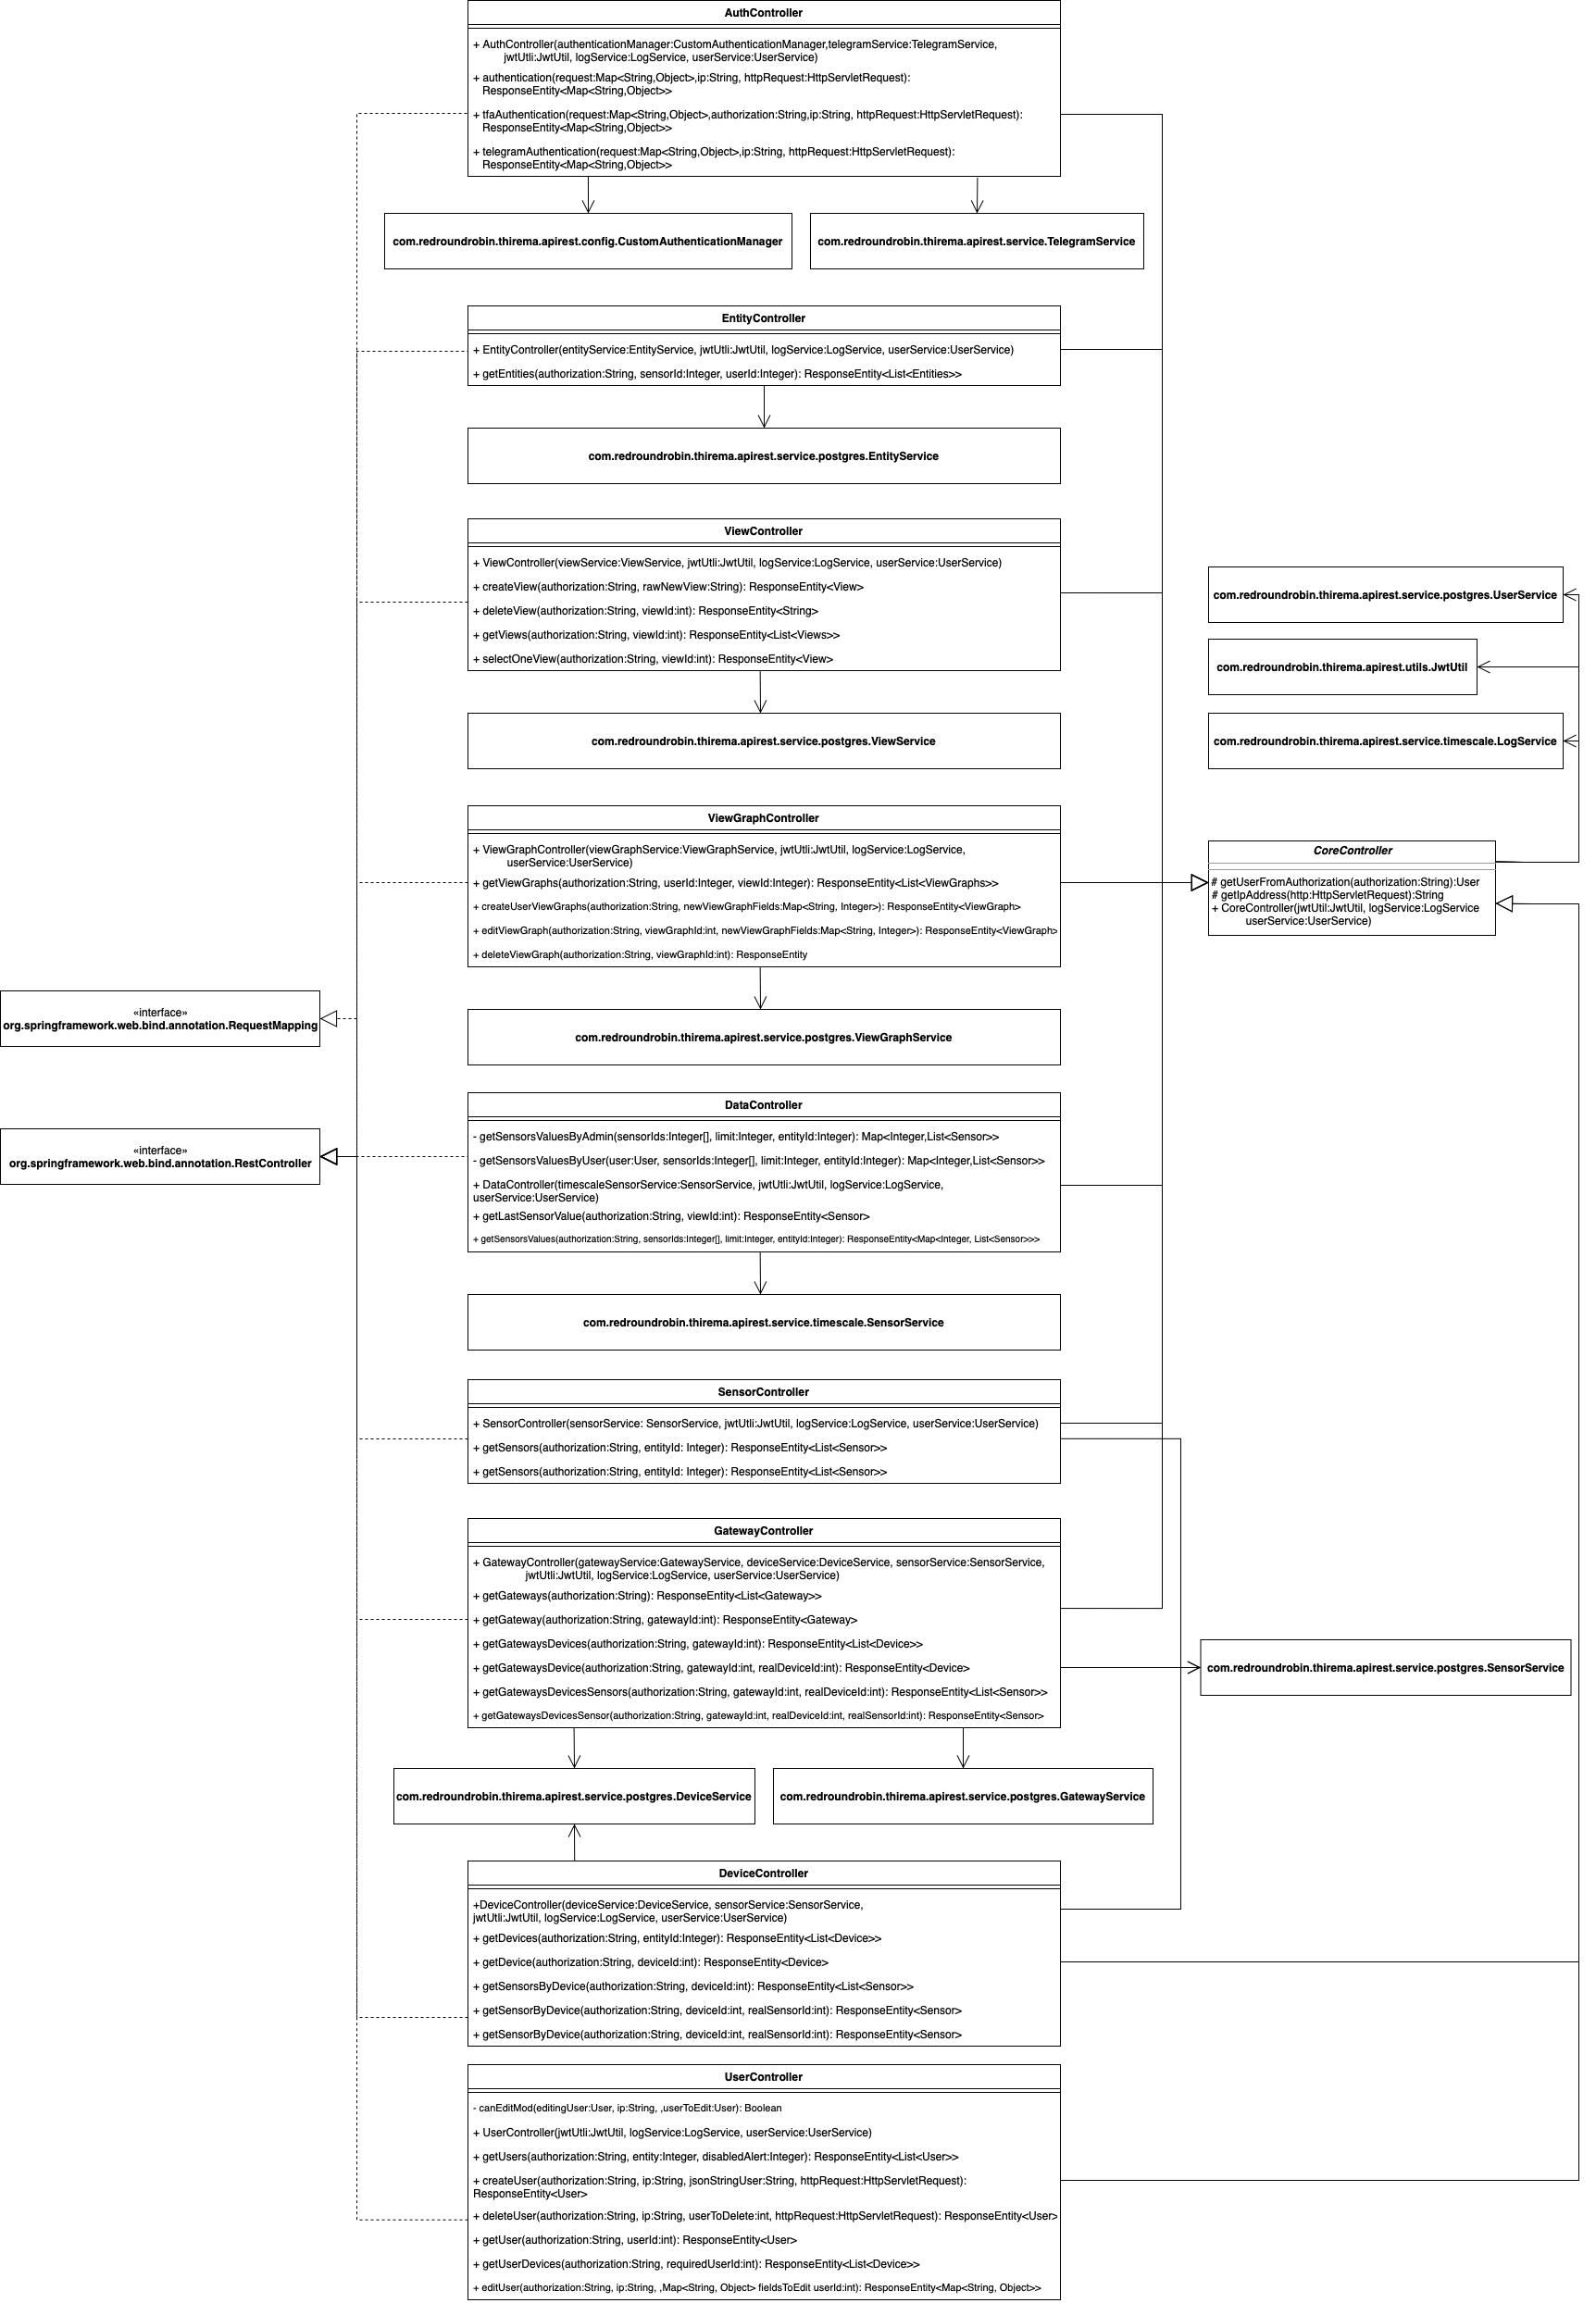
\includegraphics[scale=0.300]{res/images/API/Controllers.png}
			\caption{Diagramma del package Controllers della componente Api}
		\end{figure}
		\begin{landscape}
		\begin{figure}[H]
			\centering
			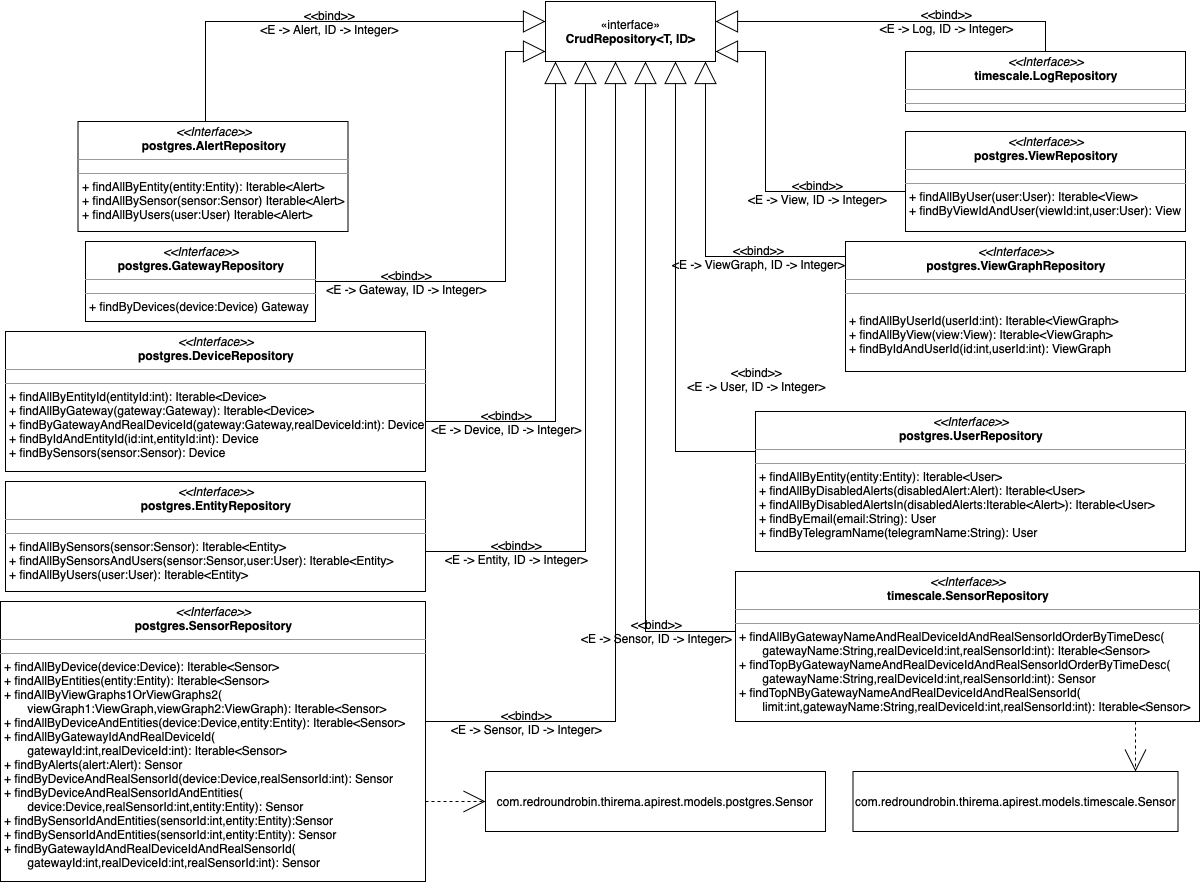
\includegraphics[scale=0.550]{res/images/API/RepositoryPackage.png}
			\caption{Diagramma del package Repository della componente Api}
		\end{figure}
		\begin{figure}[H]
			\centering
			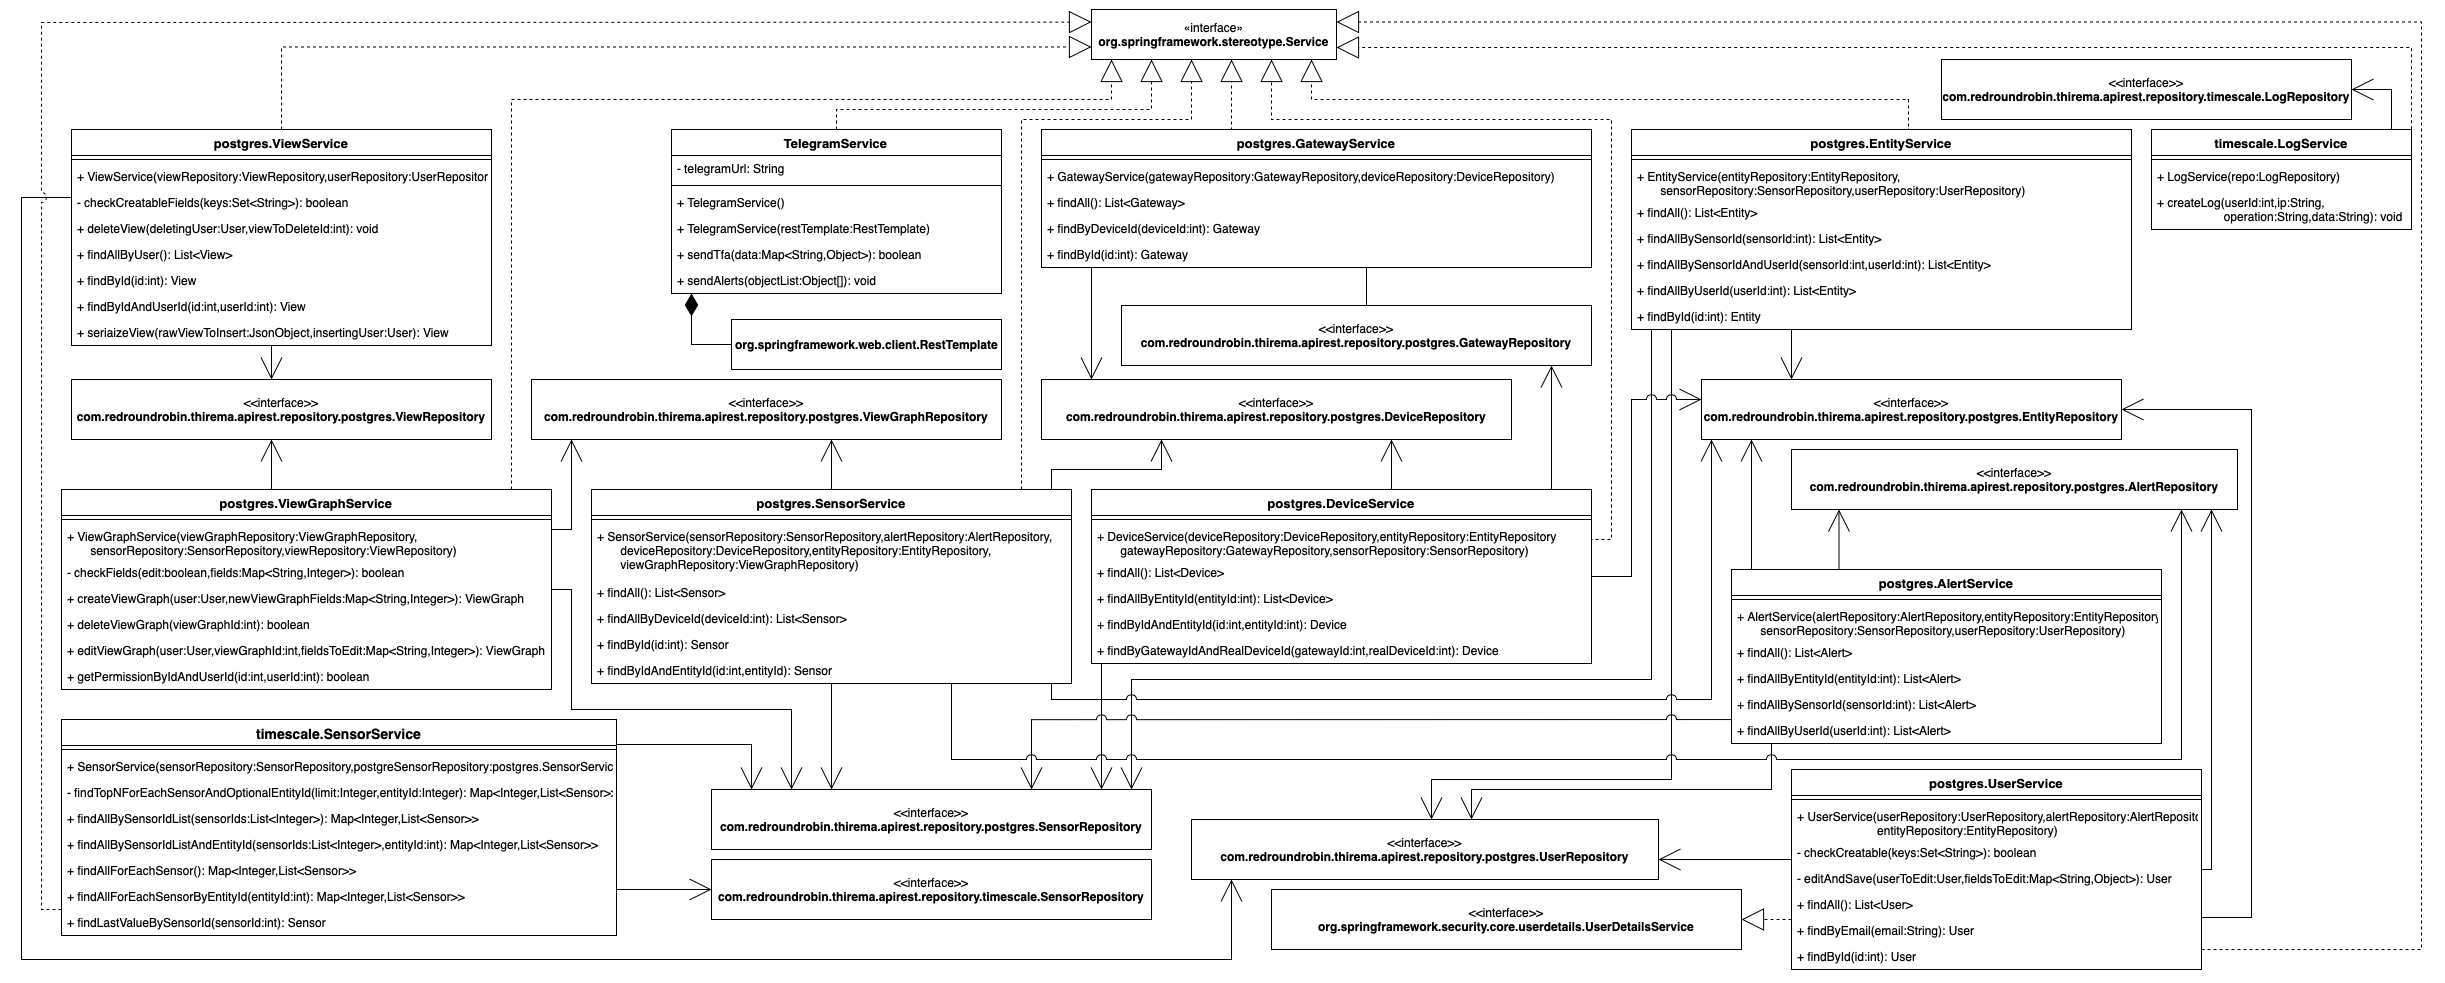
\includegraphics[scale=0.300]{res/images/API/ServicePackage.png}
			\caption{Diagramma del package Service della componente Api}
		\end{figure}
		
	\subsubsection{Diagrammi di sequenza}
		\begin{figure}[H]
			\centering
			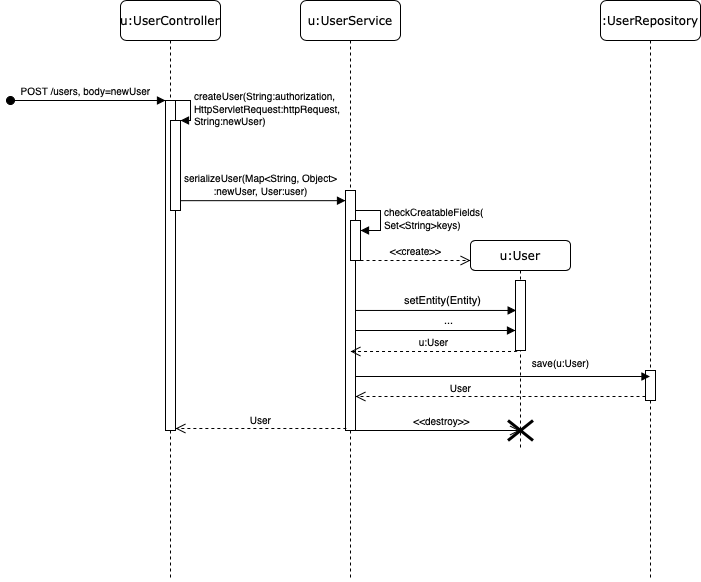
\includegraphics[scale=0.550]{res/images/API/inserimento_utente.png}
			\caption{Diagramma di sequenza che mostra l'inserimento di un utente all'interno della componente Api}
		\end{figure}
		\begin{figure}[H]
			\centering
			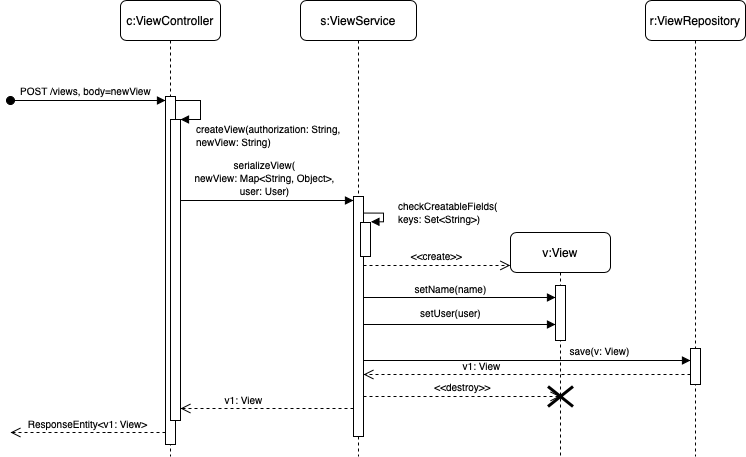
\includegraphics[scale=0.550]{res/images/API/inserimento_view.png}
			\caption{Diagramma di sequenza che mostra l'inserimento di una view all'interno della componente Api}
		\end{figure}
	\end{landscape}

